\documentclass[ignorenonframetext,]{beamer}
\usetheme{AnnArbor}
\usecolortheme{dolphin}
\usefonttheme{structurebold}
\setbeamertemplate{caption}[numbered]
\setbeamertemplate{caption label separator}{:}
\setbeamercolor{caption name}{fg=normal text.fg}
\usepackage{amssymb,amsmath}
\usepackage{ifxetex,ifluatex}
\usepackage{fixltx2e} % provides \textsubscript
\usepackage{lmodern}
\ifxetex
  \usepackage{fontspec,xltxtra,xunicode}
  \defaultfontfeatures{Mapping=tex-text,Scale=MatchLowercase}
  \newcommand{\euro}{€}
\else
  \ifluatex
    \usepackage{fontspec}
    \defaultfontfeatures{Mapping=tex-text,Scale=MatchLowercase}
    \newcommand{\euro}{€}
  \else
    \usepackage[T1]{fontenc}
    \usepackage[utf8]{inputenc}
      \fi
\fi
% use upquote if available, for straight quotes in verbatim environments
\IfFileExists{upquote.sty}{\usepackage{upquote}}{}
% use microtype if available
\IfFileExists{microtype.sty}{\usepackage{microtype}}{}
\usepackage{color}
\usepackage{fancyvrb}
\newcommand{\VerbBar}{|}
\newcommand{\VERB}{\Verb[commandchars=\\\{\}]}
\DefineVerbatimEnvironment{Highlighting}{Verbatim}{commandchars=\\\{\}}
% Add ',fontsize=\small' for more characters per line
\usepackage{framed}
\definecolor{shadecolor}{RGB}{248,248,248}
\newenvironment{Shaded}{\begin{snugshade}}{\end{snugshade}}
\newcommand{\KeywordTok}[1]{\textcolor[rgb]{0.13,0.29,0.53}{\textbf{{#1}}}}
\newcommand{\DataTypeTok}[1]{\textcolor[rgb]{0.13,0.29,0.53}{{#1}}}
\newcommand{\DecValTok}[1]{\textcolor[rgb]{0.00,0.00,0.81}{{#1}}}
\newcommand{\BaseNTok}[1]{\textcolor[rgb]{0.00,0.00,0.81}{{#1}}}
\newcommand{\FloatTok}[1]{\textcolor[rgb]{0.00,0.00,0.81}{{#1}}}
\newcommand{\CharTok}[1]{\textcolor[rgb]{0.31,0.60,0.02}{{#1}}}
\newcommand{\StringTok}[1]{\textcolor[rgb]{0.31,0.60,0.02}{{#1}}}
\newcommand{\CommentTok}[1]{\textcolor[rgb]{0.56,0.35,0.01}{\textit{{#1}}}}
\newcommand{\OtherTok}[1]{\textcolor[rgb]{0.56,0.35,0.01}{{#1}}}
\newcommand{\AlertTok}[1]{\textcolor[rgb]{0.94,0.16,0.16}{{#1}}}
\newcommand{\FunctionTok}[1]{\textcolor[rgb]{0.00,0.00,0.00}{{#1}}}
\newcommand{\RegionMarkerTok}[1]{{#1}}
\newcommand{\ErrorTok}[1]{\textbf{{#1}}}
\newcommand{\NormalTok}[1]{{#1}}
\usepackage{longtable,booktabs}
\usepackage{caption}
% These lines are needed to make table captions work with longtable:
\makeatletter
\def\fnum@table{\tablename~\thetable}
\makeatother
\usepackage{graphicx}
\makeatletter
\def\maxwidth{\ifdim\Gin@nat@width>\linewidth\linewidth\else\Gin@nat@width\fi}
\def\maxheight{\ifdim\Gin@nat@height>\textheight0.8\textheight\else\Gin@nat@height\fi}
\makeatother
% Scale images if necessary, so that they will not overflow the page
% margins by default, and it is still possible to overwrite the defaults
% using explicit options in \includegraphics[width, height, ...]{}
\setkeys{Gin}{width=\maxwidth,height=\maxheight,keepaspectratio}

% Comment these out if you don't want a slide with just the
% part/section/subsection/subsubsection title:
\AtBeginPart{
  \let\insertpartnumber\relax
  \let\partname\relax
  \frame{\partpage}
}
\AtBeginSection{
  \let\insertsectionnumber\relax
  \let\sectionname\relax
  \frame{\sectionpage}
}
\AtBeginSubsection{
  \let\insertsubsectionnumber\relax
  \let\subsectionname\relax
  \frame{\subsectionpage}
}

\setlength{\parindent}{0pt}
\setlength{\parskip}{6pt plus 2pt minus 1pt}
\setlength{\emergencystretch}{3em}  % prevent overfull lines
\providecommand{\tightlist}{%
  \setlength{\itemsep}{0pt}\setlength{\parskip}{0pt}}
\setcounter{secnumdepth}{0}
\pgfdeclareimage[height=0.1cm, width=1cm]{logo}{}
\logo{\pgfuseimage{logo}}
\institute{}
\definecolor{links}{HTML}{2A1B81}
\definecolor{mypink2}{RGB}{219, 48, 122}
\hypersetup{colorlinks,linkcolor=links,urlcolor=mypink2}
\usefonttheme{professionalfonts}
\setbeamerfont{note page}{family*=pplx,size=\footnotesize} % Palatino for notes
\usepackage{helvet}
\useinnertheme{rectangles}

\title[Lung imaging and ANTs]{Neuroimaging with ANTs as a model for the pulmonary community}
\author{Jim Gee}
\date{}

\begin{document}
\frame{\titlepage}

\begin{frame}
\tableofcontents[subsectionsonly]
\end{frame}

\section{Significance}\label{significance}

\begin{frame}{E. A. Hoffman et al., JMRI 2015.}

\begin{quote}
``More widespread use of all {[}pulmonary{]} imaging biomarkers has been
limited for a number of key reasons, including: 1) lack of support to
harmonize image acquisition software; \textbf{2) universally available
image analysis software;} 3) regulatory boundaries for emerging
approaches; and 4) historically weak links between respiratory and
radiology clinical programs.''
\end{quote}

\end{frame}

\begin{frame}{What does the neuroimaging community offer?}

Great packages such as:

\begin{itemize}
\itemsep1pt\parskip0pt\parsep0pt
\item
  AFNI
\item
  FSL
\item
  FreeSurfer
\item
  SPM
\end{itemize}

\end{frame}

\begin{frame}{Public \& robust software $\longrightarrow$ research
output}

\includegraphics{stitchedSlides_files/figure-beamer/pubmedQuery-1.pdf}

\end{frame}

\begin{frame}{Benefits of open-source:}

\begin{itemize}
\itemsep1pt\parskip0pt\parsep0pt
\item
  Motivates community-based support:

  \begin{itemize}
  \itemsep1pt\parskip0pt\parsep0pt
  \item
    bug fixes (\emph{``Given enough eyeballs, all bugs are shallow.''}),
  \item
    new features,
  \item
    reproducibility verification, and
  \item
    community tech support.
  \end{itemize}
\item
  Learn directly from journal manuscripts \emph{and} implementations.
\item
  Tremendous cost-savings.
\end{itemize}

\end{frame}

\section{Innovation}\label{innovation}

\section{Preliminary data}\label{preliminary-data}

\section{ANTs functionality}\label{ants-functionality}

\begin{frame}{Donoho?}

 \emph{``Papers are just advertisements for the science.''}

\end{frame}

\begin{frame}{ANTs core tools}

\begin{itemize}
\itemsep1pt\parskip0pt\parsep0pt
\item
  image registration
\item
  template building
\item
  Bayesian segmentation with priors
\item
  N4 bias correction
\item
  joint label fusion
\item
  spatially adaptive denoising
\end{itemize}

\end{frame}

\begin{frame}{Symmetric Normalization (SyN)}

$\int_{t=0}^{0.5} \left(\|\mathbf{v}_1(x,t)\|_L^2 + \|\mathbf{v}_2(x,t)\|_L^2\right)dt + \|I\left(\phi_1(x,0.5)\right) - J_i\left(\phi_2(x,0.5)\right)\|^2$

\includegraphics{./Figs/fishes.png}

\end{frame}

\begin{frame}{Diffeomorphisms: Occam's razor modeling}

\includegraphics{./Figs/sillyputty.png}

\emph{differentiable map with differentiable inverse}

\end{frame}

\begin{frame}{Diffeomoprhisms: fine-grained and flexible maps}

\includegraphics{./Figs/highresdiffeos.jpg}

\end{frame}

\begin{frame}{Beyond original SyN}

\small

\includegraphics{./Figs/Frontiers_ITK.png}

\includegraphics{./Figs/Frontiers_BSplineSyN.png}

\end{frame}

\begin{frame}[fragile]{\texttt{antsRegistration}}

\begin{Shaded}
\begin{Highlighting}[]
\NormalTok{$ }\KeywordTok{antsRegistration} \NormalTok{-h}

\KeywordTok{COMMAND}\NormalTok{:}
     \KeywordTok{antsRegistration}

\KeywordTok{OPTIONS}\NormalTok{:}
     \KeywordTok{--version}
     \KeywordTok{-d}\NormalTok{, --dimensionality 2/3}
     \KeywordTok{-o}\NormalTok{, --output outputTransformPrefix}
                  \NormalTok{[}\KeywordTok{outputTransformPrefix}\NormalTok{,}\KeywordTok{<}\NormalTok{outputWarpedImage}\KeywordTok{>}\NormalTok{,}\KeywordTok{<}\NormalTok{outputInverseWarpedImage}\KeywordTok{>}\NormalTok{]}
     \KeywordTok{-j}\NormalTok{, --save-state saveSateAsTransform}
     \KeywordTok{-k}\NormalTok{, --restore-state restoreStateAsATransform}
     \KeywordTok{-a}\NormalTok{, --write-composite-transform 1/(0)}
     \KeywordTok{-p}\NormalTok{, --print-similarity-measure-interval }\KeywordTok{<}\NormalTok{unsignedIntegerValue}\KeywordTok{>}
     \KeywordTok{--write-interval-volumes} \KeywordTok{<}\NormalTok{unsignedIntegerValue}\KeywordTok{>}
     \KeywordTok{-z}\NormalTok{, --collapse-output-transforms (1)}\KeywordTok{/0}
     \KeywordTok{-i}\NormalTok{, --initialize-transforms-per-stage (1)}\KeywordTok{/0}
     \KeywordTok{-n}\NormalTok{, --interpolation Linear}
                         \KeywordTok{NearestNeighbor}
                         \KeywordTok{MultiLabel}\NormalTok{[}\KeywordTok{<}\NormalTok{sigma=imageSpacing}\KeywordTok{>}\NormalTok{,}\KeywordTok{<}\NormalTok{alpha=4.}\KeywordTok{0>}\NormalTok{]}
                         \KeywordTok{Gaussian}\NormalTok{[}\KeywordTok{<}\NormalTok{sigma=imageSpacing}\KeywordTok{>}\NormalTok{,}\KeywordTok{<}\NormalTok{alpha=1.}\KeywordTok{0>}\NormalTok{]}
                         \KeywordTok{BSpline}\NormalTok{[}\KeywordTok{<}\NormalTok{order=}\KeywordTok{3>}\NormalTok{]}
                         \KeywordTok{CosineWindowedSinc}
                         \KeywordTok{WelchWindowedSinc}
                         \KeywordTok{HammingWindowedSinc}
                         \KeywordTok{LanczosWindowedSinc}
     \KeywordTok{-g}\NormalTok{, --restrict-deformation PxQxR}
     \KeywordTok{-q}\NormalTok{, --initial-fixed-transform initialTransform}
                                   \NormalTok{[}\KeywordTok{initialTransform}\NormalTok{,}\KeywordTok{<}\NormalTok{useInverse}\KeywordTok{>}\NormalTok{]}
                                   \NormalTok{[}\KeywordTok{fixedImage}\NormalTok{,movingImage,initializationFeature]}
     \KeywordTok{-r}\NormalTok{, --initial-moving-transform initialTransform}
                                    \NormalTok{[}\KeywordTok{initialTransform}\NormalTok{,}\KeywordTok{<}\NormalTok{useInverse}\KeywordTok{>}\NormalTok{]}
                                    \NormalTok{[}\KeywordTok{fixedImage}\NormalTok{,movingImage,initializationFeature]}
     \KeywordTok{-m}\NormalTok{, --metric CC[fixedImage,movingImage,metricWeight,radius,}\KeywordTok{<}\NormalTok{samplingStrategy=}\DataTypeTok{\{None,Regular,Random\}}\KeywordTok{>}\NormalTok{,}\KeywordTok{<}\NormalTok{samplingPercentage=[0,1]}\KeywordTok{>}\NormalTok{]}
                  \KeywordTok{MI}\NormalTok{[fixedImage,movingImage,metricWeight,numberOfBins,}\KeywordTok{<}\NormalTok{samplingStrategy=}\DataTypeTok{\{None,Regular,Random\}}\KeywordTok{>}\NormalTok{,}\KeywordTok{<}\NormalTok{samplingPercentage=[0,1]}\KeywordTok{>}\NormalTok{]}
                  \KeywordTok{Mattes}\NormalTok{[fixedImage,movingImage,metricWeight,numberOfBins,}\KeywordTok{<}\NormalTok{samplingStrategy=}\DataTypeTok{\{None,Regular,Random\}}\KeywordTok{>}\NormalTok{,}\KeywordTok{<}\NormalTok{samplingPercentage=[0,1]}\KeywordTok{>}\NormalTok{]}
                  \KeywordTok{MeanSquares}\NormalTok{[fixedImage,movingImage,metricWeight,radius=NA,}\KeywordTok{<}\NormalTok{samplingStrategy=}\DataTypeTok{\{None,Regular,Random\}}\KeywordTok{>}\NormalTok{,}\KeywordTok{<}\NormalTok{samplingPercentage=[0,1]}\KeywordTok{>}\NormalTok{]}
                  \KeywordTok{Demons}\NormalTok{[fixedImage,movingImage,metricWeight,radius=NA,}\KeywordTok{<}\NormalTok{samplingStrategy=}\DataTypeTok{\{None,Regular,Random\}}\KeywordTok{>}\NormalTok{,}\KeywordTok{<}\NormalTok{samplingPercentage=[0,1]}\KeywordTok{>}\NormalTok{]}
                  \KeywordTok{GC}\NormalTok{[fixedImage,movingImage,metricWeight,radius=NA,}\KeywordTok{<}\NormalTok{samplingStrategy=}\DataTypeTok{\{None,Regular,Random\}}\KeywordTok{>}\NormalTok{,}\KeywordTok{<}\NormalTok{samplingPercentage=[0,1]}\KeywordTok{>}\NormalTok{]}
                  \KeywordTok{ICP}\NormalTok{[fixedPointSet,movingPointSet,metricWeight,}\KeywordTok{<}\NormalTok{samplingPercentage=[0,1]}\KeywordTok{>}\NormalTok{,}\KeywordTok{<}\NormalTok{boundaryPointsOnly=}\KeywordTok{0>}\NormalTok{]}
                  \KeywordTok{PSE}\NormalTok{[fixedPointSet,movingPointSet,metricWeight,}\KeywordTok{<}\NormalTok{samplingPercentage=[0,1]}\KeywordTok{>}\NormalTok{,}\KeywordTok{<}\NormalTok{boundaryPointsOnly=}\KeywordTok{0>}\NormalTok{,}\KeywordTok{<}\NormalTok{pointSetSigma=}\KeywordTok{1>}\NormalTok{,}\KeywordTok{<}\NormalTok{kNeighborhood=}\KeywordTok{50>}\NormalTok{]}
                  \KeywordTok{JHCT}\NormalTok{[fixedPointSet,movingPointSet,metricWeight,}\KeywordTok{<}\NormalTok{samplingPercentage=[0,1]}\KeywordTok{>}\NormalTok{,}\KeywordTok{<}\NormalTok{boundaryPointsOnly=}\KeywordTok{0>}\NormalTok{,}\KeywordTok{<}\NormalTok{pointSetSigma=}\KeywordTok{1>}\NormalTok{,}\KeywordTok{<}\NormalTok{kNeighborhood=}\KeywordTok{50>}\NormalTok{,}\KeywordTok{<}\NormalTok{alpha=1.}\KeywordTok{1>}\NormalTok{,}\KeywordTok{<}\NormalTok{useAnisotropicCovariances=}\KeywordTok{1>}\NormalTok{]}
                  \KeywordTok{IGDM}\NormalTok{[fixedImage,movingImage,metricWeight,fixedMask,movingMask,}\KeywordTok{<}\NormalTok{neighborhoodRadius=0x}\KeywordTok{0>}\NormalTok{,}\KeywordTok{<}\NormalTok{intensitySigma=}\KeywordTok{0>}\NormalTok{,}\KeywordTok{<}\NormalTok{distanceSigma=}\KeywordTok{0>}\NormalTok{,}\KeywordTok{<}\NormalTok{kNeighborhood=}\KeywordTok{1>}\NormalTok{,}\KeywordTok{<}\NormalTok{gradientSigma=}\KeywordTok{1>}\NormalTok{]}
     \KeywordTok{-t}\NormalTok{, --transform Rigid[gradientStep]}
                     \KeywordTok{Affine}\NormalTok{[gradientStep]}
                     \KeywordTok{CompositeAffine}\NormalTok{[gradientStep]}
                     \KeywordTok{Similarity}\NormalTok{[gradientStep]}
                     \KeywordTok{Translation}\NormalTok{[gradientStep]}
                     \KeywordTok{BSpline}\NormalTok{[gradientStep,meshSizeAtBaseLevel]}
                     \KeywordTok{GaussianDisplacementField}\NormalTok{[gradientStep,updateFieldVarianceInVoxelSpace,totalFieldVarianceInVoxelSpace]}
                     \KeywordTok{BSplineDisplacementField}\NormalTok{[gradientStep,updateFieldMeshSizeAtBaseLevel,totalFieldMeshSizeAtBaseLevel,}\KeywordTok{<}\NormalTok{splineOrder=}\KeywordTok{3>}\NormalTok{]}
                     \KeywordTok{TimeVaryingVelocityField}\NormalTok{[gradientStep,numberOfTimeIndices,updateFieldVarianceInVoxelSpace,updateFieldTimeVariance,totalFieldVarianceInVoxelSpace,totalFieldTimeVariance]}
                     \KeywordTok{TimeVaryingBSplineVelocityField}\NormalTok{[gradientStep,velocityFieldMeshSize,}\KeywordTok{<}\NormalTok{numberOfTimePointSamples=}\KeywordTok{4>}\NormalTok{,}\KeywordTok{<}\NormalTok{splineOrder=}\KeywordTok{3>}\NormalTok{]}
                     \KeywordTok{SyN}\NormalTok{[gradientStep,updateFieldVarianceInVoxelSpace,totalFieldVarianceInVoxelSpace]}
                     \KeywordTok{BSplineSyN}\NormalTok{[gradientStep,updateFieldMeshSizeAtBaseLevel,totalFieldMeshSizeAtBaseLevel,}\KeywordTok{<}\NormalTok{splineOrder=}\KeywordTok{3>}\NormalTok{]}
                     \KeywordTok{Exponential}\NormalTok{[gradientStep,updateFieldVarianceInVoxelSpace,velocityFieldVarianceInVoxelSpace,}\KeywordTok{<}\NormalTok{numberOfIntegrationSteps}\KeywordTok{>}\NormalTok{]}
                     \KeywordTok{BSplineExponential}\NormalTok{[gradientStep,updateFieldMeshSizeAtBaseLevel,velocityFieldMeshSizeAtBaseLevel,}\KeywordTok{<}\NormalTok{numberOfIntegrationSteps}\KeywordTok{>}\NormalTok{,}\KeywordTok{<}\NormalTok{splineOrder=}\KeywordTok{3>}\NormalTok{]}
     \KeywordTok{-c}\NormalTok{, --convergence MxNxO}
                       \NormalTok{[}\KeywordTok{MxNxO}\NormalTok{,}\KeywordTok{<}\NormalTok{convergenceThreshold=1e-}\KeywordTok{6>}\NormalTok{,}\KeywordTok{<}\NormalTok{convergenceWindowSize=}\KeywordTok{10>}\NormalTok{]}
     \KeywordTok{-s}\NormalTok{, --smoothing-sigmas MxNxO...}
     \KeywordTok{-f}\NormalTok{, --shrink-factors MxNxO...}
     \KeywordTok{-u}\NormalTok{, --use-histogram-matching}
     \KeywordTok{-l}\NormalTok{, --use-estimate-learning-rate-once}
     \KeywordTok{-w}\NormalTok{, --winsorize-image-intensities [lowerQuantile,upperQuantile]}
     \KeywordTok{-x}\NormalTok{, --masks [fixedImageMask,movingImageMask]}
     \KeywordTok{--float}
     \KeywordTok{--minc}
     \KeywordTok{-v}\NormalTok{, --verbose (0)}\KeywordTok{/1}
     \KeywordTok{-h}
     \KeywordTok{--help}
\end{Highlighting}
\end{Shaded}

\end{frame}

\begin{frame}{Template building: creating the average Joe}

\includegraphics{./Figs/template0.jpg}

\end{frame}

\begin{frame}{``Attractiveness'' $\rightarrow$ mental processing?}

\includegraphics{./Figs/template1.jpg}

\end{frame}

\begin{frame}{What about brains?}

\includegraphics{./Figs/template3.jpg}

\end{frame}

\begin{frame}{Templates facilitate computation}

\includegraphics{./Figs/template4.jpg}

\end{frame}

\begin{frame}{Gender discernibility?}

\includegraphics{./Figs/template5.jpg}

\end{frame}

\begin{frame}[fragile]{\texttt{antsMultivariateTemplateConstruction2.sh}}

\begin{Shaded}
\begin{Highlighting}[]
\NormalTok{$ }\KeywordTok{antsMultivariateTemplateConstruction2.sh}

\KeywordTok{Usage}\NormalTok{:}

\KeywordTok{antsMultivariateTemplateConstruction2.sh} \NormalTok{-d ImageDimension -o OutputPrefix }\KeywordTok{<}\NormalTok{other options}\KeywordTok{>} \KeywordTok{<}\NormalTok{images}\KeywordTok{>}

\KeywordTok{Compulsory} \NormalTok{arguments (minimal command line requires SGE/PBS cluster, otherwise use -c and}
  \KeywordTok{-j} \NormalTok{options)}\KeywordTok{:}

     \KeywordTok{-d}\NormalTok{:  ImageDimension: 2 or 3 (for 2 or 3 dimensional registration of single volume)}
   \KeywordTok{ImageDimension}\NormalTok{: 4 (for template generation of time-series data)}

     \KeywordTok{-o}\NormalTok{:  OutputPrefix}\KeywordTok{;} \KeywordTok{A} \NormalTok{prefix that is prepended to all output files.}

\KeywordTok{<images>}  \NormalTok{List of images in the current directory, eg *_t1.nii.gz. Should be at the end}
          \KeywordTok{of} \NormalTok{the command.  Optionally, one can specify a .csv or .txt file where each}
          \KeywordTok{line} \NormalTok{is the location of the input image.  One can also specify more than}
          \KeywordTok{one} \NormalTok{file for each image for multi-modal template construction (e.g. t1 and t2)}\KeywordTok{.}
          \KeywordTok{For} \NormalTok{the multi-modal case, the templates will be consecutively numbered (e.g.}
          \KeywordTok{template0.nii.gz}\NormalTok{, template1.nii.gz, ...)}\KeywordTok{.}

\KeywordTok{NB}\NormalTok{: All images to be added to the template should be in the same directory, and this}
    \KeywordTok{script} \NormalTok{should be invoked from that directory.}

\KeywordTok{Optional} \NormalTok{arguments:}

     \KeywordTok{-a}   \NormalTok{image statistic used to summarize images (default 1)}
          \KeywordTok{0} \NormalTok{= mean}
          \KeywordTok{1} \NormalTok{= mean of normalized intensities}
          \KeywordTok{2} \NormalTok{= median}

     \KeywordTok{-b}\NormalTok{:  Backup images and results from all iterations (default = 0)}\KeywordTok{:}  \NormalTok{Boolean to save}
          \KeywordTok{the} \NormalTok{transform files, bias corrected, and warped images for each iteration.}

     \KeywordTok{-c}\NormalTok{:  Control for parallel computation (default 0)}\KeywordTok{:}
          \KeywordTok{0} \NormalTok{= run serially}
          \KeywordTok{1} \NormalTok{= SGE qsub}
          \KeywordTok{2} \NormalTok{= use PEXEC (localhost)}
          \KeywordTok{3} \NormalTok{= Apple XGrid}
          \KeywordTok{4} \NormalTok{= PBS qsub}

     \KeywordTok{-e}   \NormalTok{use single precision ( default 1 )}

     \KeywordTok{-g}\NormalTok{:  Gradient step size (default 0.25)}\KeywordTok{:} \NormalTok{smaller in magnitude results in more}
          \KeywordTok{cautious} \NormalTok{steps.}

     \KeywordTok{-i}\NormalTok{:  Iteration limit (default 4)}\KeywordTok{:} \NormalTok{iterations of the template construction}
          \KeywordTok{(Iteration} \NormalTok{limit}\KeywordTok{)*NumImages} \NormalTok{registrations.}

     \KeywordTok{-j}\NormalTok{:  Number of cpu cores to use locally for pexec option (default 2}\KeywordTok{;} \KeywordTok{requires} \StringTok{"-c 2"}\NormalTok{)}

     \KeywordTok{-k}\NormalTok{:  Number of modalities used to construct the template (default 1)}\KeywordTok{:}  \NormalTok{For example,}
          \KeywordTok{if} \KeywordTok{one} \NormalTok{wanted to create a multimodal template consisting of T1,T2,and FA}
          \KeywordTok{components} \NormalTok{(}\StringTok{"-k 3"}\NormalTok{)}\KeywordTok{.}

     \KeywordTok{-w}\NormalTok{:  Modality weights used in the similarity metric (default = 1)}\KeywordTok{:} \NormalTok{specified as}
          \KeywordTok{e.g.} \NormalTok{1x0.5x0.75.}

     \KeywordTok{-q}\NormalTok{:  Max iterations for each pairwise registration (default = 100x100x70x20)}\KeywordTok{:}
          \KeywordTok{specified} \NormalTok{in the form ...xJxKxL where}
            \KeywordTok{J} \NormalTok{= max iterations at coarsest resolution (here, reduced by power of 2^2)}
            \KeywordTok{K} \NormalTok{= middle resolution iterations (here, reduced by power of 2)}
            \KeywordTok{L} \NormalTok{= fine resolution iteratioxns (here, full resolution)}\KeywordTok{.}
          \KeywordTok{Finer} \NormalTok{resolutions take much more time per iteration than coarser resolutions.}

     \KeywordTok{-f}\NormalTok{:  Shrink factors (default = 6x4x2x1)}\KeywordTok{:}  \NormalTok{Also in the same form as -q max iterations.}
          \KeywordTok{Needs} \NormalTok{to have the same number of components.}

     \KeywordTok{-s}\NormalTok{:  Smoothing factors (default = 3x2x1x0)}\KeywordTok{:}  \NormalTok{Also in the same form as -q max}
          \KeywordTok{iterations.}  \NormalTok{Needs to have the same number of components.}

     \KeywordTok{-n}\NormalTok{:  N4BiasFieldCorrection of moving image: 0 == off, 1 == on (default 1)}\KeywordTok{.}

     \KeywordTok{-p}\NormalTok{:  Commands to prepend to job scripts (e.g., change into appropriate directory, set}
          \KeywordTok{paths}\NormalTok{, etc)}

     \KeywordTok{-r}\NormalTok{:  Do rigid-body registration of inputs before creating template (default 0)}\KeywordTok{:}
          \KeywordTok{0} \NormalTok{== off 1 == on. Only useful when you do not have an initial template}

     \KeywordTok{-l}\NormalTok{:  Use linear image registration stages during the pairwise (template/subject)}
          \KeywordTok{deformable} \NormalTok{registration.  Otherwise, registration is limited to SyN or}
          \KeywordTok{B-spline} \NormalTok{SyN (see }\StringTok{'-t'} \NormalTok{option)}\KeywordTok{.}  \KeywordTok{This} \NormalTok{is }\StringTok{'1'} \NormalTok{by default.}

     \KeywordTok{-m}\NormalTok{:  Type of similarity metric used for registration (default = CC)}\KeywordTok{:}  \NormalTok{Options are}
            \KeywordTok{CC} \NormalTok{= cross-correlation}
            \KeywordTok{MI} \NormalTok{= mutual information}
            \KeywordTok{MSQ} \NormalTok{= mean square difference}
            \KeywordTok{DEMONS} \NormalTok{= demon}\StringTok{'s metric}
\StringTok{          A similarity metric per modality can be specified.  If the CC metric is chosen,}
\StringTok{          one can also specify the radius in brackets, e.g. '}\NormalTok{-m CC[4]}\StringTok{'.}

\StringTok{     -t:  Type of transformation model used for registration (default = SyN):  Options are}
\StringTok{            SyN = Greedy SyN}
\StringTok{            BSplineSyN = Greedy B-spline SyN}
\StringTok{            TimeVaryingVelocityField = Time-varying velocity field}
\StringTok{            TimeVaryingBSplineVelocityField = Time-varying B-spline velocity field}

\StringTok{     -u:  Walltime (default = 20:00:00):  Option for PBS qsub specifying requested time}
\StringTok{          per pairwise registration.}

\StringTok{     -v:  Memory limit (default = 8gb):  Option for PBS qsub specifying requested memory}
\StringTok{          per pairwise registration.}

\StringTok{     -x:  XGrid arguments (e.g., -x "-p password -h controlhost")}

\StringTok{     -y:  Update the template with the full affine transform (default 1). If 0, the rigid}
\StringTok{          component of the affine transform will not be used to update the template. If your}
\StringTok{          template drifts in translation or orientation try -y 0.}

\StringTok{     -z:  Use this this volume as the target of all inputs. When not used, the script}
\StringTok{          will create an unbiased starting point by averaging all inputs. Use the full}
\StringTok{          path.}
\StringTok{          For multiple modalities, specify -z modality1.nii.gz -z modality2.nii.gz ...}
\StringTok{          in the same modality order as the input images.}

\StringTok{Example:}

\StringTok{antsMultivariateTemplateConstruction2.sh -d 3 -i 3 -k 1 -f 4x2x1 -s 2x1x0vox -q 30x20x4 -t SyN  -m CC -c 0 -o MY sub*avg.nii.gz}

\StringTok{Multimodal example:}

\StringTok{antsMultivariateTemplateConstruction2.sh -d 3 -i 3 -k 2 -f 4x2x1 -s 2x1x0vox -q 30x20x4 -t SyN -z t1.nii.gz -z t2.nii.gz  -m CC -c 0 -o MY templateInput.csv}

\StringTok{where templateInput.csv contains}

\StringTok{subjectA_t1.nii.gz,subjectA_t2.nii.gz}
\StringTok{subjectB_t1.nii.gz,subjectB_t2.nii.gz}
\StringTok{...}

\StringTok{--------------------------------------------------------------------------------------}
\StringTok{ANTS was created by:}
\StringTok{--------------------------------------------------------------------------------------}
\StringTok{Brian B. Avants, Nick Tustison and Gang Song}
\StringTok{Penn Image Computing And Science Laboratory}
\StringTok{University of Pennsylvania}

\StringTok{Please reference http://www.ncbi.nlm.nih.gov/pubmed/20851191 when employing this script}
\StringTok{in your studies. A reproducible evaluation of ANTs similarity metric performance in}
\StringTok{brain image registration:}

\StringTok{* Avants BB, Tustison NJ, Song G, Cook PA, Klein A, Gee JC. Neuroimage, 2011.}

\StringTok{Also see http://www.ncbi.nlm.nih.gov/pubmed/19818860 for more details.}

\StringTok{The script has been updated and improved since this publication.}

\StringTok{--------------------------------------------------------------------------------------}
\StringTok{Script by Nick Tustison}
\StringTok{--------------------------------------------------------------------------------------}
\StringTok{Apple XGrid support by Craig Stark}
\StringTok{--------------------------------------------------------------------------------------}
\end{Highlighting}
\end{Shaded}

\end{frame}

\begin{frame}{Bayesian segmentation with spatial/MRF priors}

\end{frame}

\begin{frame}{``20+ years of development. \emph{Show me the code!}''}

Brian Avants, MICCAI workshop

\end{frame}

\begin{frame}{Atropos}

\includegraphics{./Figs/atropos.png}

\end{frame}

\begin{frame}{Algorithmic workflow(Atropos + N4)}

\includegraphics{./Figs/atroposFlow.png}

\end{frame}

\begin{frame}{Sample results from public data}

\includegraphics{./Figs/sampleAtroposVisualResults.png}

\end{frame}

\begin{frame}[fragile]{Command line help}

\begin{verbatim}
$ Atropos -h

COMMAND:
     Atropos

OPTIONS:
     -d, --image-dimensionality 2/3/4
     -a, --intensity-image [intensityImage,<adaptiveSmoothingWeight>]
     -b, --bspline [<numberOfLevels=6>,<initialMeshResolution=1x1x...>,<splineOrder=3>]
     -i, --initialization Random[numberOfClasses]
                          Otsu[numberOfTissueClasses]
                          KMeans[numberOfTissueClasses,<clusterCenters(in ascending order and for first intensity image only)>]
                          PriorProbabilityImages[numberOfTissueClasses,fileSeriesFormat(index=1 to numberOfClasses) or vectorImage,priorWeighting,<priorProbabilityThreshold>]
                          PriorLabelImage[numberOfTissueClasses,labelImage,priorWeighting]
     -s, --partial-volume-label-set label1xlabel2xlabel3
     --use-partial-volume-likelihoods 1/(0)
                                      true/(false)
     -p, --posterior-formulation Socrates[<useMixtureModelProportions=1>,<initialAnnealingTemperature=1>,<annealingRate=1>,<minimumTemperature=0.1>]
                                 Plato[<useMixtureModelProportions=1>,<initialAnnealingTemperature=1>,<annealingRate=1>,<minimumTemperature=0.1>]
                                 Aristotle[<useMixtureModelProportions=1>,<initialAnnealingTemperature=1>,<annealingRate=1>,<minimumTemperature=0.1>]
                                 Sigmoid[<useMixtureModelProportions=1>,<initialAnnealingTemperature=1>,<annealingRate=1>,<minimumTemperature=0.1>]]
     -x, --mask-image maskImageFilename
     -c, --convergence [<numberOfIterations=5>,<convergenceThreshold=0.001>]
     -k, --likelihood-model Gaussian
                            HistogramParzenWindows[<sigma=1.0>,<numberOfBins=32>]
                            ManifoldParzenWindows[<pointSetSigma=1.0>,<evaluationKNeighborhood=50>,<CovarianceKNeighborhood=0>,<kernelSigma=0>]
                            JointShapeAndOrientationProbability[<shapeSigma=1.0>,<numberOfShapeBins=64>, <orientationSigma=1.0>, <numberOfOrientationBins=32>]
                            LogEuclideanGaussian
     -m, --mrf [<smoothingFactor=0.3>,<radius=1x1x...>]
               [<mrfCoefficientImage>,<radius=1x1x...>]
     -g, --icm [<useAsynchronousUpdate=1>,<maximumNumberOfICMIterations=1>,<icmCodeImage=''>]
     -r, --use-random-seed 0/(1)
     -o, --output [classifiedImage,<posteriorProbabilityImageFileNameFormat>]
     -u, --minimize-memory-usage (0)/1
     -w, --winsorize-outliers BoxPlot[<lowerPercentile=0.25>,<upperPercentile=0.75>,<whiskerLength=1.5>]
                              GrubbsRosner[<significanceLevel=0.05>,<winsorizingLevel=0.10>]
     -e, --use-euclidean-distance (0)/1
     -l, --label-propagation whichLabel[lambda=0.0,<boundaryProbability=1.0>]
     -h
     --help
\end{verbatim}

\end{frame}

\begin{frame}{N4 bias correction}

\end{frame}

\begin{frame}{Nonparametric nonuniform intensity normalization (N3)}

\begin{itemize}
\item
  Developed at the Montreal Neurological Institute (John Sled, 1998)
\item
  Part of the standard preprocessing protocol in large scale projects
  such as ADNI
\item
  The traditional de facto standard in MRI bias correction

  \begin{itemize}
  \itemsep1pt\parskip0pt\parsep0pt
  \item
    good performance
  \item
    \emph{public availability}
  \end{itemize}
\item
  Public availability --- set of perl scripts coordinating various C++
  programs
\item
  ``\emph{Let's incorporate N3 into ANTs!}''
\end{itemize}

\end{frame}

\begin{frame}{N3 adoption issues}

\includegraphics{./Figs/whyN4.png}

``\emph{So let's re-implement N3 in ITK for ANTs users.}''

\end{frame}

\begin{frame}{N3 -\textgreater{} N4*}

*Nick's N3

\begin{itemize}
\item
  comparative
  \href{http://www.ncbi.nlm.nih.gov/pubmed/20378467}{evaluation}
\item
  smaller spline distances (useful for higher magnet strengths)
\item
  multiresolution
\item
  weighted regional mask (used in
  \href{https://github.com/stnava/ANTs/blob/master/Scripts/antsAtroposN4.sh}{\texttt{antsAtroposN4.sh}})
\item
  faster execution times
\item
  less susceptible to noise
\item
  \emph{publicly available}
\end{itemize}

\end{frame}

\begin{frame}{N4 example}

\includegraphics{./Figs/KKI2009_MPRAGE_slice150.png}

\end{frame}

\begin{frame}[fragile]{Command line help}

\begin{verbatim}
$ N4BiasFieldCorrection -h

COMMAND:
     N4BiasFieldCorrection

OPTIONS:
     -d, --image-dimensionality 2/3/4
     -i, --input-image inputImageFilename
     -x, --mask-image maskImageFilename
     -r, --rescale-intensities 0/(1)
     -w, --weight-image weightImageFilename
     -s, --shrink-factor 1/2/3/4/...
     -c, --convergence [<numberOfIterations=50x50x50x50>,<convergenceThreshold=0.0>]
     -b, --bspline-fitting [splineDistance,<splineOrder=3>]
                           [initialMeshResolution,<splineOrder=3>]
     -t, --histogram-sharpening [<FWHM=0.15>,<wienerNoise=0.01>,<numberOfHistogramBins=200>]
     -o, --output correctedImage
                  [correctedImage,<biasField>]
     -h
     --help
\end{verbatim}

\end{frame}

\begin{frame}{Joint label fusion}

\end{frame}

\begin{frame}{Multi-atlas labeling}

\includegraphics{./competitions/figures/NKI30_MALF.png}

\end{frame}

\begin{frame}{Multi-atlas segmentation}

\includegraphics{./Figs/jointLabelFusion.png}

\end{frame}

\begin{frame}{Multi-atlas 2012 results}

\includegraphics{./competitions/figures/MALF2012.png}

\end{frame}

\begin{frame}{New work: joint intensity fusion}

\includegraphics{./Figs/jointIntensityFusion.png}

\end{frame}

\begin{frame}[fragile]{Command line help}

\begin{verbatim}
$ antsJointFusion -h

COMMAND:
     antsJointFusion

OPTIONS:
     -d, --image-dimensionality 2/3/4
     -t, --target-image targetImage
                        [targetImageModality0,targetImageModality1,...,targetImageModalityN]
     -g, --atlas-image atlasImage
                       [atlasImageModality0,atlasImageModality1,...,atlasImageModalityN]
     -l, --atlas-segmentation atlasSegmentation
     -a, --alpha 0.1
     -b, --beta 2.0
     -r, --retain-label-posterior-images (0)/1
     -f, --retain-atlas-voting-images (0)/1
     -c, --constrain-nonnegative (0)/1
     -p, --patch-radius 2
                        2x2x2
     -m, --patch-metric (PC)/MSQ
     -s, --search-radius 3
                         3x3x3
     -e, --exclusion-image label[exclusionImage]
     -x, --mask-image maskImageFilename
     -o, --output labelFusionImage
                  intensityFusionImageFileNameFormat
                  [labelFusionImage,intensityFusionImageFileNameFormat,<labelPosteriorProbabilityImageFileNameFormat>,<atlasVotingWeightImageFileNameFormat>]
     --version
     -v, --verbose (0)/1
     -h
     --help
\end{verbatim}

\end{frame}

\begin{frame}{Spatially adaptive denoising}

\end{frame}

\begin{frame}[fragile]{Command line help}

\begin{verbatim}
$ DenoiseImage -h

COMMAND:
     DenoiseImage

OPTIONS:
     -d, --image-dimensionality 2/3/4
     -i, --input-image inputImageFilename
     -n, --noise-model Rician/(Gaussian)
     -s, --shrink-factor (1)/2/3/...
     -o, --output correctedImage
                  [correctedImage,<noiseImage>]
     --version
     -v, --verbose (0)/1
     -h
     --help
\end{verbatim}

\end{frame}

\section{Algorithmic competition}\label{algorithmic-competition}

\begin{frame}{International competitions}

\begin{itemize}
\itemsep1pt\parskip0pt\parsep0pt
\item
  \href{http://www.ncbi.nlm.nih.gov/pubmed/19195496}{Klein 2009}
\item
  \href{http://empire10.isi.uu.nl}{EMPIRE 2010}
\item
  \href{https://masi.vuse.vanderbilt.edu/workshop2012/index.php/Main_Page}{Multi-Atlas
  Label Challenge 2012}
\item
  \href{https://masi.vuse.vanderbilt.edu/workshop2013/index.php/MICCAI_2013_SATA_Challenge_and_Workshop:Current_events}{SATA
  Challenge 2013}
\item
  \href{http://martinos.org/qtim/miccai2013/}{BRATS 2013}
\item
  \href{http://www.cardiacatlas.org/web/stacom2014/moco-introduction}{STACOM
  2014 MoCo Challenge}
\end{itemize}

\end{frame}

\begin{frame}{Klein, NeuroImage 2009}

\includegraphics{./competitions/figures/nihms-130679-f0001.jpg}

\end{frame}

\begin{frame}{Klein results}

\includegraphics{./competitions/figures/KleinResults2009.png}

\end{frame}

\begin{frame}{Take-away message}

\emph{``One of the most significant findings of this study is that the
relative performances of the registration methods under comparison
appear to be little affected by the choice of subject population,
labeling protocol, and type of overlap measure\ldots{}. ART, SyN, IRTK,
and SPM's DARTEL Toolbox gave the best results according to overlap and
distance measures, with ART and SyN delivering the most consistently
high accuracy across subjects and label sets.''}

\end{frame}

\begin{frame}{EMPIRE 2010}

\includegraphics{./competitions/figures/EMPIRE10criteria.png}

\begin{itemize}
\item
  Alignment of lung boundaries,
\item
  major fissures,
\item
  annotated landmark pairs, and
\item
  topology of displacement field.
\end{itemize}

\end{frame}

\begin{frame}{EMPIRE 2010 results}

\includegraphics{./competitions/figures/EMPIRE10Results.png}

\end{frame}

\begin{frame}{Multi-atlas 2012}

\includegraphics{./competitions/figures/NKI30_MALF.png}

\end{frame}

\begin{frame}{Multi-atlas 2012 results}

\includegraphics{./competitions/figures/MALF2012.png}

\end{frame}

\begin{frame}{SATA 2013}

Three very different problem domains

\includegraphics{./competitions/figures/SATA_data.png}

\end{frame}

\begin{frame}{BRATS 2013}

\includegraphics{./competitions/figures/brats2013results1.png}

\end{frame}

\begin{frame}{BRATS 2013 results}

{\textbf{Results}}

\includegraphics{./competitions/figures/brats2013results2.png}

Optimal symmetric multimodal templates and concatenated random forests
for supervised brain tumor segmentation (simplified) with ANTsR,
\emph{Neuroinformatics}.

\end{frame}

\begin{frame}{STACOM 2014}

\includegraphics{./competitions/figures/image_gallery.jpg}

\end{frame}

\section{ANTs for neuroimaging}\label{ants-for-neuroimaging}

\section{Putting it all together---the ANTs cortical thickness
pipeline}\label{putting-it-all-togetherthe-ants-cortical-thickness-pipeline}

\begin{frame}{Cortical thickness studies}

\begin{longtable}[c]{@{}ll@{}}
\toprule\addlinespace
Column1 & Column2
\\\addlinespace
\midrule\endhead
Tetris-playing ability & chronic pancreatitis
\\\addlinespace
Huntington's disease & obsessive-compulsive disorder
\\\addlinespace
schizophrenia & ADHD
\\\addlinespace
bipolar disorder & obesity
\\\addlinespace
Alzheimer's disease & heritable depression
\\\addlinespace
frontotemporal dementia & elderly depression
\\\addlinespace
Parkinson's disease & age
\\\addlinespace
Williams syndrome & gender
\\\addlinespace
multiple sclerosis & handedness
\\\addlinespace
autism & intelligence
\\\addlinespace
migraines & athletic ability
\\\addlinespace
chronic smoking & meditative practices
\\\addlinespace
alcoholism & musical ability
\\\addlinespace
cocaine addiction & tendency toward criminality
\\\addlinespace
Tourette syndrome in children & childhood sexual abuse in female
adolescents
\\\addlinespace
scoliosis in female adolescents & traumatic brain injury
\\\addlinespace
early-onset blindness & untreated male-to-female transsexuality
\\\addlinespace
\bottomrule
\end{longtable}

\end{frame}

\begin{frame}{Basic components of the pipeline}

\begin{enumerate}
\def\labelenumi{\arabic{enumi}.}
\itemsep1pt\parskip0pt\parsep0pt
\item
  template building (offline)
\item
  brain extraction
\item
  cortical thickness estimation
\item
  cortical parcellation
\end{enumerate}

\end{frame}

\begin{frame}{Sample results}

\includegraphics{./evaluation/figures/components.png}

\end{frame}

\begin{frame}{The ANTs structural brain mapping workflow}

\includegraphics{./evaluation/figures/pipeline.png}

\end{frame}

\begin{frame}{Template building}

\emph{Tailor data to your specific cohort}

\includegraphics{./evaluation/figures/templates.png}

\end{frame}

\begin{frame}{Template priors}

\includegraphics{./evaluation/figures/templatePriors.png}

\end{frame}

\begin{frame}{Cortical thickness estimation}

\includegraphics{./evaluation/figures/corticalThicknessEstimation.png}

\end{frame}

\begin{frame}{\emph{But without ground truth, how does one evaluate the
pipeline?}}

\end{frame}

\begin{frame}{Predict age and gender}

$AGE \sim VOLUME + GENDER + \sum_{i=1}^{62} T(DKT_i)$

\end{frame}

\begin{frame}{Open science principles}

\includegraphics{./evaluation/figures/ageDistribution.png}

\end{frame}

\begin{frame}{Prediction from cortical thickness data}

\includegraphics{./evaluation/figures/evaluation.png}

\end{frame}

\begin{frame}{Age prediction per site}

\includegraphics{./evaluation/figures/agePredictionPerSite.png}

\end{frame}

\begin{frame}{Regional importance comparison}

\includegraphics{./evaluation/figures/antsvfreesurfer_Importance.png}

ANTs (left) vs.~FreeSurfer (right)

\end{frame}

\begin{frame}{Regional measurements}

\includegraphics{./evaluation/figures/antsvfreesurfer_regionalPlots.png}

\end{frame}

\section{ANTs for pulmonary imaging}\label{ants-for-pulmonary-imaging}

\begin{frame}{ANTs core tools for lung image analysis}

\includegraphics{./lung/figures/coreANtsToolsLung.png}

\end{frame}

\begin{frame}{Functional ventilation}

\includegraphics{./lung/figures/prePostAlbuterol.png}

\end{frame}

\begin{frame}{Lung and lobe estimation}

\includegraphics{./lung/figures/lungEstimation.png}

\end{frame}

\begin{frame}{Good results on 1H MRI}

\begin{longtable}[c]{@{}lccc@{}}
\toprule\addlinespace
& \textbf{Mean} & \textbf{SD} & \textbf{Median}
\\\addlinespace
\midrule\endhead
\textbf{Left lung} & 0.963 (0.974) & 0.013 (0.097) & 0.964 (0.992)
\\\addlinespace
\textbf{Right lung} & 0.968 (0.972) & 0.012 (0.135) & 0.970 (0.996)
\\\addlinespace
\textbf{Left upper} & 0.882 (0.922) & 0.059 (0.163) & 0.894 (0.978)
\\\addlinespace
\textbf{Left lower} & 0.868 (0.885) & 0.06 (0.229) & 0.892 (0.964)
\\\addlinespace
\textbf{Right upper} & 0.852 (0.921) & 0.067 (0.088) & 0.875 (0.96)
\\\addlinespace
\textbf{Right middle} & 0.657 (0.765) & 0.130 (0.299) & 0.696 (0.886)
\\\addlinespace
\textbf{Right lower} & 0.873 (0.914) & 0.063 (0.176) & 0.900 (0.968)
\\\addlinespace
\bottomrule
\end{longtable}

(*) Comparison with state-of-the-art in both 1H MRI and CT

\end{frame}

\begin{frame}{Combining ANTs lung functionality I}

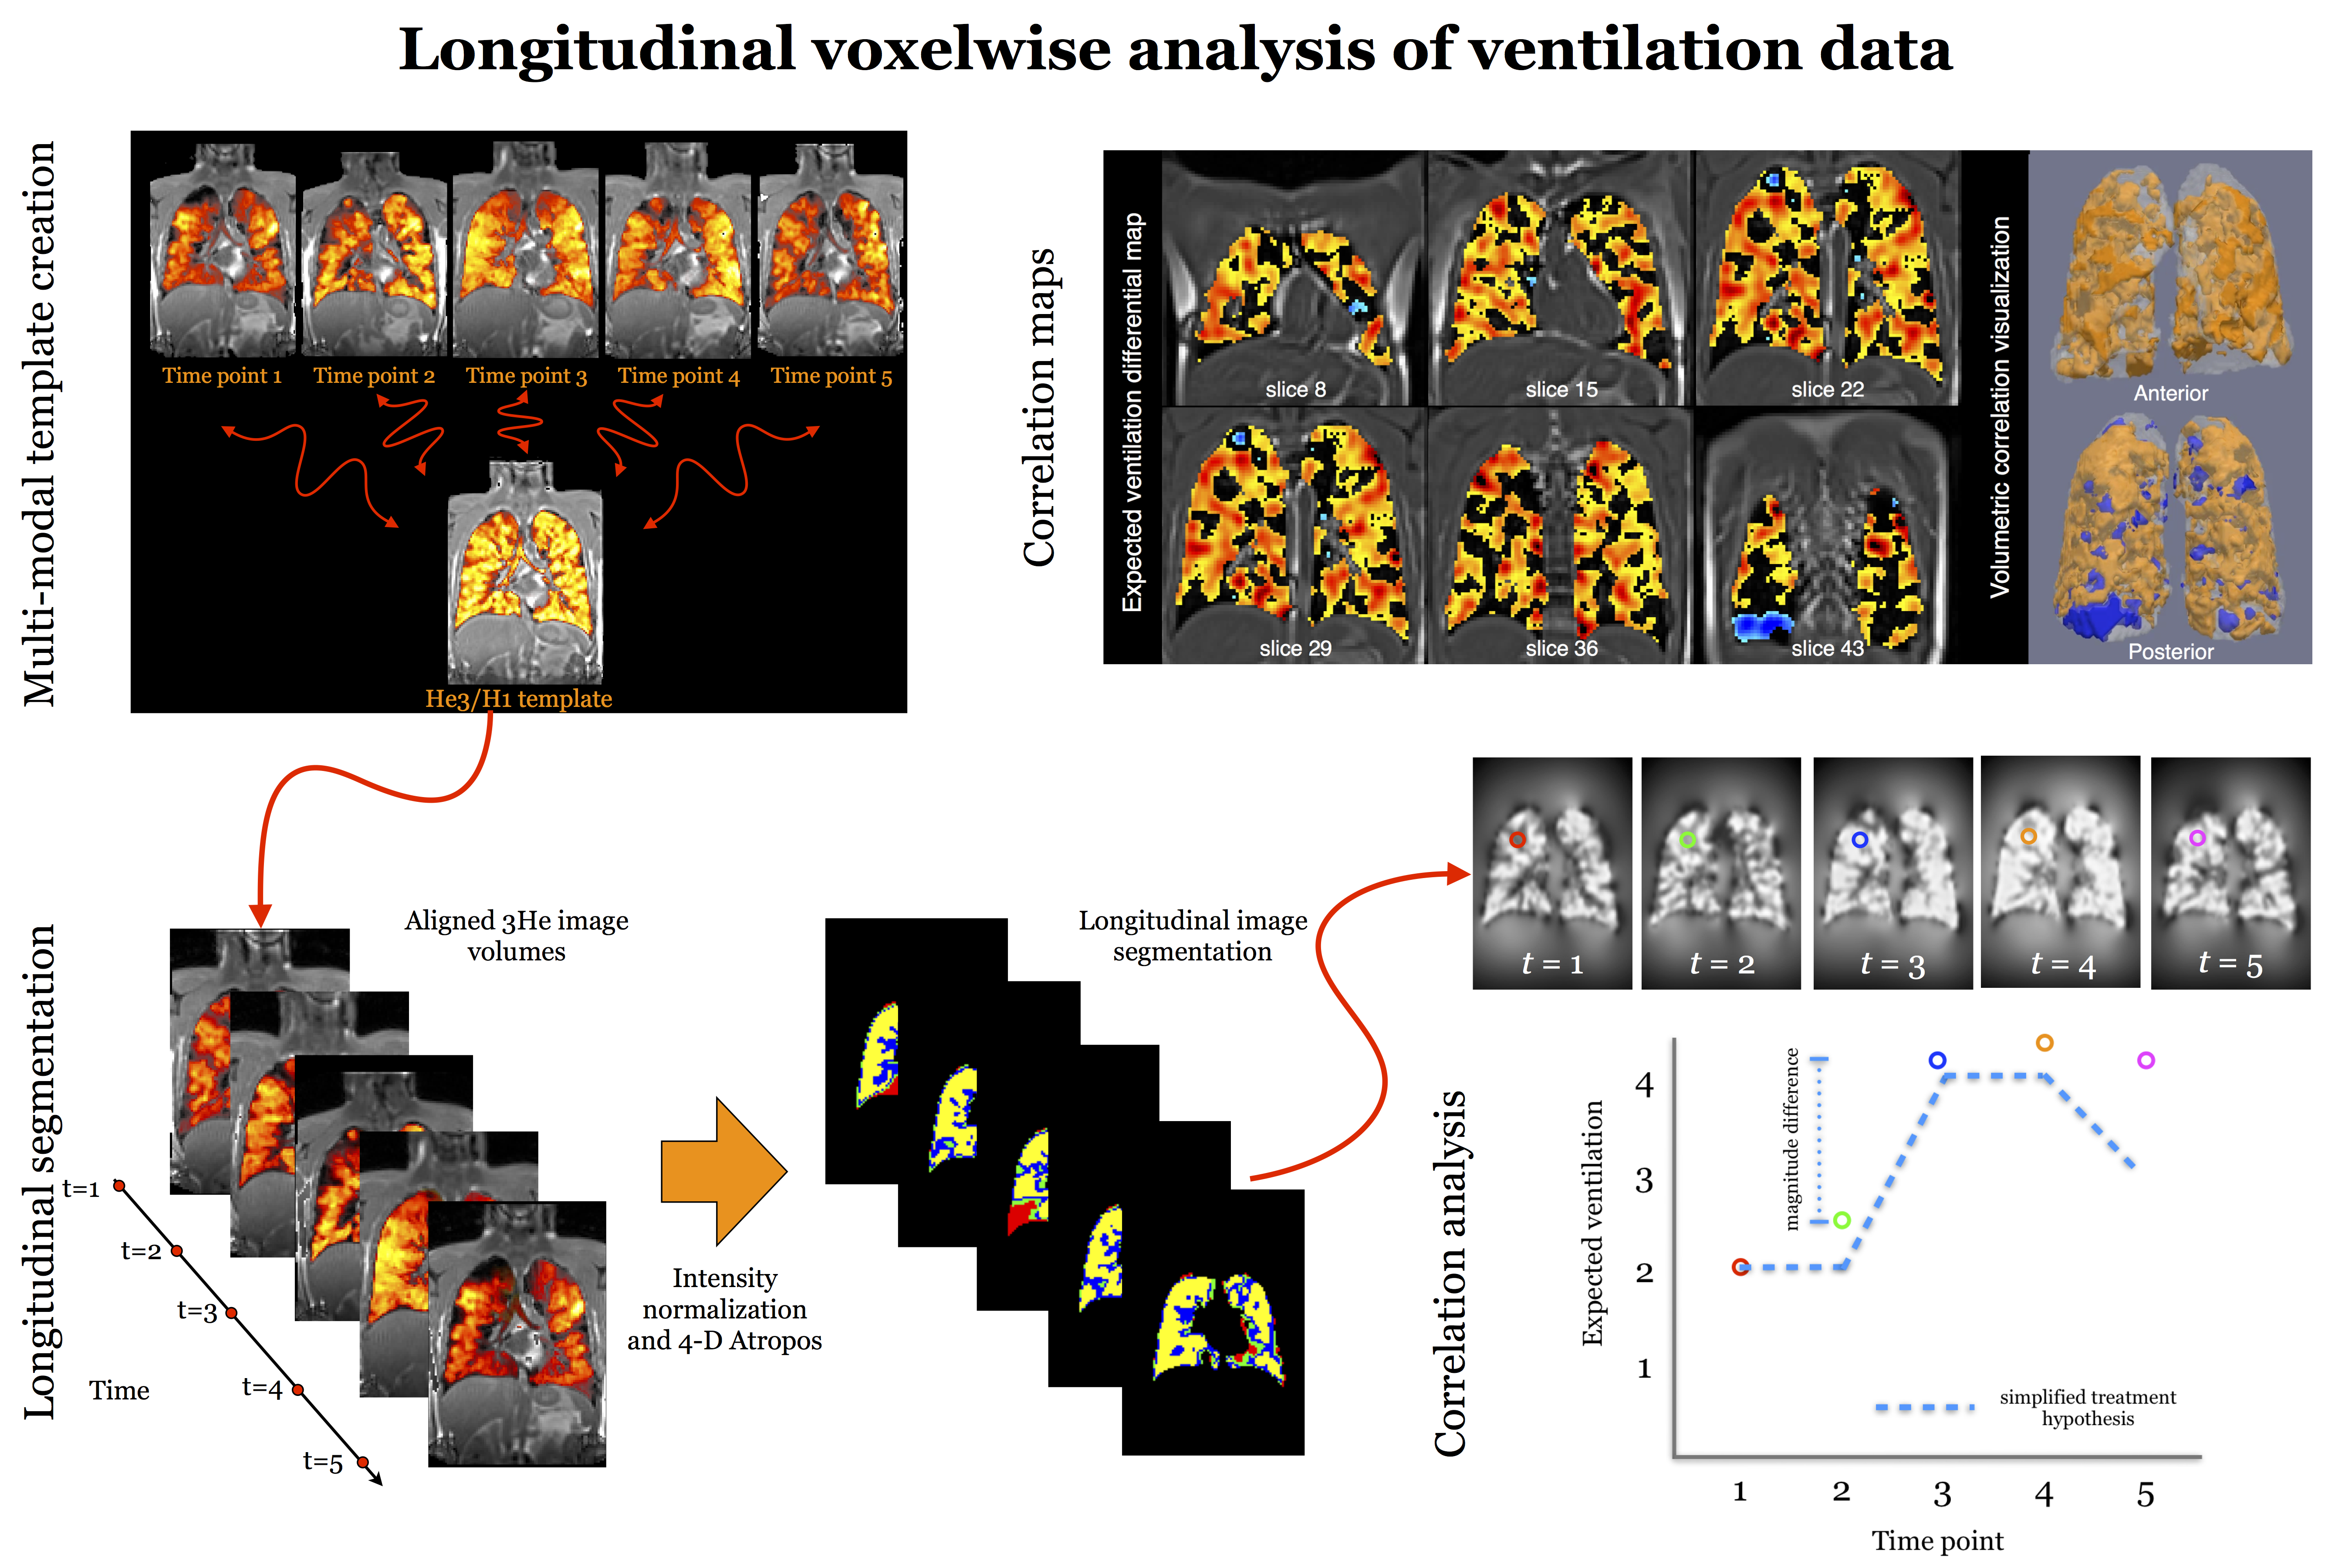
\includegraphics{./lung/figures/longitudinalStudy.png}

\end{frame}

\begin{frame}{Combining ANTs lung functionality II}

\includegraphics{./lung/figures/airways.png}

\end{frame}

\end{document}